\documentclass[12pt,twoside]{rif}

\pagestyle{myheadings}
\usepackage[
left=2.54cm,
right=2.54cm,
top=2.54cm,
bottom=2.54cm]
{geometry}
\usepackage{hyperref}
\usepackage{natbib}
\usepackage{subfigure}
\hypersetup{
	urlcolor=blue, 
	colorlinks=true, 
	citecolor=blue
}

\usepackage{lipsum}

\title{\textbf{Dilatación del tiempo gravitacional}}

\author[1]{{\small Carlos Andrés García Suarez}} 
\author[1]{{\small David Brandon Zevallos Garay}}
\author[1]{{\small Luis Fernando Ubillus Benites}}
%\author[3]{Autor3}
\affil[1]{{ \small Facultad de Ciencias Naturales y Matemática, Universidad
		Nacional Federico Villarreal. El Agustino 15003. Lima-Perú.}}
%\affil[2,3]{Afiliacion2}
%\date{\normalsize Recibido: xxxx Aceptado: xxxx Publicado: xxxx\\
%Todos los derechos reservados-SEF \copyright{} 2012}
\date{}

\begin{document}
	\maketitle
	
	\begin{res}
		\begin{center}
			\textbf{Resumen} \\
		\end{center}
		\lipsum[2]
		
		\par
		\smallskip
		\clav{sdjssasdfsdf, asdfsdf, asdfsdafsd}
	\end{res}
	\begin{center}
		\title{\textbf{Time gravitational dilation}}
	\end{center}
	
	\begin{abst}
		\begin{center}
			\textbf{Abstract} \\
		\end{center}
		\lipsum[2]
		
		\par 
		\smallskip
		\key{sdjssasdfsdf, asdfsdf, asdfsdafsd}
	\end{abst}

	
	
	\newpage
	
	\tableofcontents
	
	\section{ Introducción} 
	\subsection{Transformadas de Galileo}
	Una de los primeros indicios a nivel historico de relatividad fue propuesto 
	por Galileo, el principio de relatividad de Galileo establece que:
	Dos sistemas de referencia en movimiento relativo de traslación rectilínea 
	uniforme son equivalentes desde el punto de vista mecánico; es decir, los experimentos 
	mecánicos se desarrollan de igual manera en ambos, y las leyes de la mecánica son las mismas.

    Suponga que se presenta algún fenómeno físico, que llamará evento, el cual es observado por alguien en reposo en un marco inercial de referencia. Al decir que un observador está “en un marco”, significa que está en reposo respecto al origen de ese marco. La
    ubicación y tiempo del evento pueden ser especificados por las cuatro coordenadas (x, y,
    z, t). Lo deseable es poder transformar las coordenadas de un observador en un marco
    inercial a las de otro en un marco que se mueve con velocidad relativa uniforme en comparación con el primer marco.

	\begin{figure}[h!]
		\centering
		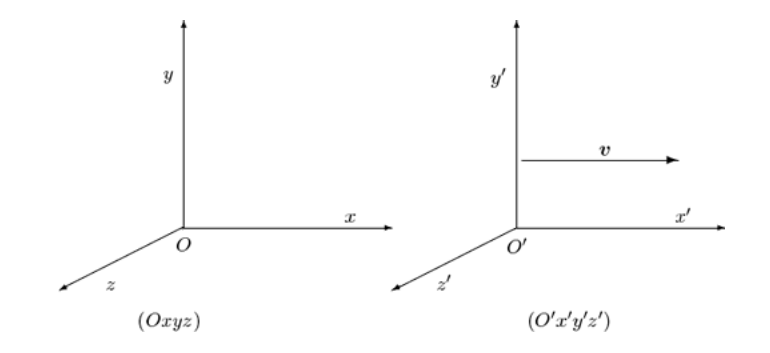
\includegraphics[width=0.7\textwidth]{img/Galileo.PNG}
		\caption{Sistemas de referencia en movimiento relativo rectilíneo
		y uniforme, con velocidad $v$ en dirección $O_{x}$ }
		\label{fig:01}
		\end{figure}

		Como muestra la geometría de la figura \ref*{fig:01}, las relaciones entre estas coordenadas se escriben 
		como:
		\begin{align*}
			x'&=x-vt\\
			y'&=y\\
			z'&=z\\
			t'&=t\\
		\end{align*}

		Éstas son las ecuaciones de transformación galileanas del espacio–tiempo. Observe que
		el tiempo se supone el mismo en ambos marcos inerciales; es decir, dentro de la estructura de la mecánica clásica, todos los relojes funcionan al mismo ritmo, cualquiera que
		sea su velocidad, de modo que el tiempo en el que se presenta un evento para un observador en S es el mismo tiempo para el mismo evento en S9. En consecuencia, el intervalo
		de tiempo entre dos eventos sucesivos debe ser el mismo para ambos observadores.
\newpage
	\subsection{Transformadas de Lorentz}

	
Según los postulados de Einstein todas las leyes físicas tienen que permanecer 
invariantes para todos los observadores con velocidad relativa constante
y la velocidad de la luz es una invariante física con el mismo valor para todos 
los observadores inerciales.Bajo estas suposiciones, la transformación de Galileo 
no es válida, en particular la ecuación $t = t' $ no puede ser correcta. Si la velocidad de la luz es la
misma para dos observadores con movimiento relativo uniforme, no es posible, 
como se verá después, que los dos midan el mismo tiempo. En otras
palabras, el intervalo de tiempo entre dos eventos no tiene por qué ser el
mismo para observadores en movimiento relativo. En definitiva debemos
reemplazar la transformación Galileana por otra, de modo que la velocidad
de la luz sea invariante.

\begin{figure}[h!]
	\centering
	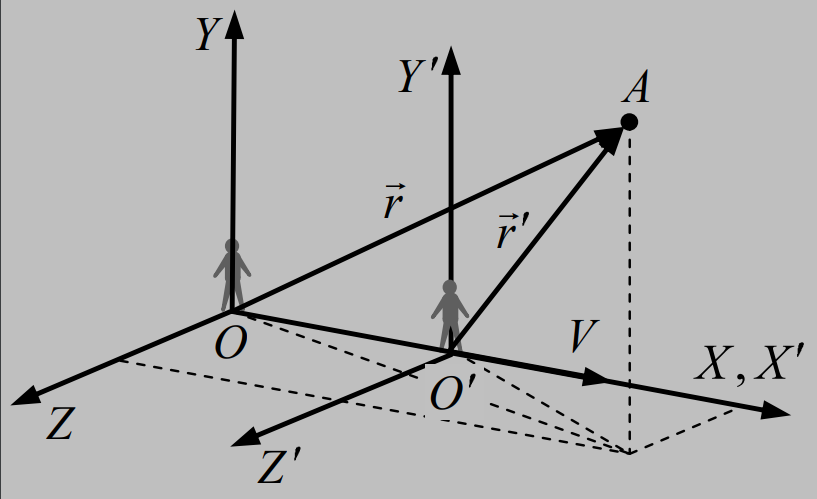
\includegraphics[width=0.7\textwidth]{img/LORENTZ.PNG}
	\caption{Sistemas de referencia de observadores inerciales }
	\label{fig:02}
	\end{figure}
	


De la figura \ref*{fig:02}	supondremos dos observadores inerciales $O$ y $O'$ de modo que $O'$ se mueve respecto a $O$ con velocidad constante V en la dirección del eje OX común de sus respectivos sistemas de coordenadas, como se ve en la figura. Exigimos 
que los dos observadores ajusten sus relojes de modo que $t = t = 0$ cuando sus posiciones coinciden.
Para $t = t = 0$ se emite un destello de luz en la
posición común (o sea, cuando $O$ y $O'$ coinciden). 

%Después de un tiempo t el
%observador $O$ notará que la luz ha llegado al punto A y escribirá $r = ct$, siendo $c$ la velocidad de la luz y $r$ la distancia que recorre desde $O$ hasta A. De la
%figura se desprende que,
%\begin{align*}
%	x^{2}+y^{2}+z^{2}=r^{2}
%\end{align*}
%or lo tanto, también se cumple que,	
%\begin{align*}
%	x^{2}+y^{2}+z^{2}=c^{2}t^{2}
%\end{align*}
Las transformaciones de Lorentz dicen que si el sistema $O'$
está en movimiento uniforme a velocidad  $v$, a lo largo del eje X del sistema $O$, y 
en el instante inicial ($t=t'=0$) el origen 
de coordenadas de ambos sistemas coinciden, entonces las coordenadas atribuidas por los 
dos observadores están relacionadas por las siguientes expresiones:
	
\begin{align*}
	x'&=\gamma(x-vt)\\
	y'&=y\\
	z'&=z\\
	t'&=\gamma(t-\frac{v}{c^{2}}x)\\
\end{align*}

Donde $\gamma$ = $\frac{1}{\sqrt{1-\frac{v^{2}}{c^{2}}}}$
	
	
	\subsection{Diagrama Minkowski}
	
	
	
	\section{Marco Teórico}

	
		
	\section{Conclusiones}
	
	\nocite{*}
	\bibliographystyle{apa}
	\bibliography{biblio}
	

\end{document}